
%(BEGIN_QUESTION)
% Copyright 2006, Tony R. Kuphaldt, released under the Creative Commons Attribution License (v 1.0)
% This means you may do almost anything with this work of mine, so long as you give me proper credit

Beskriv alt som er representert i denne P\&ID-en:

$$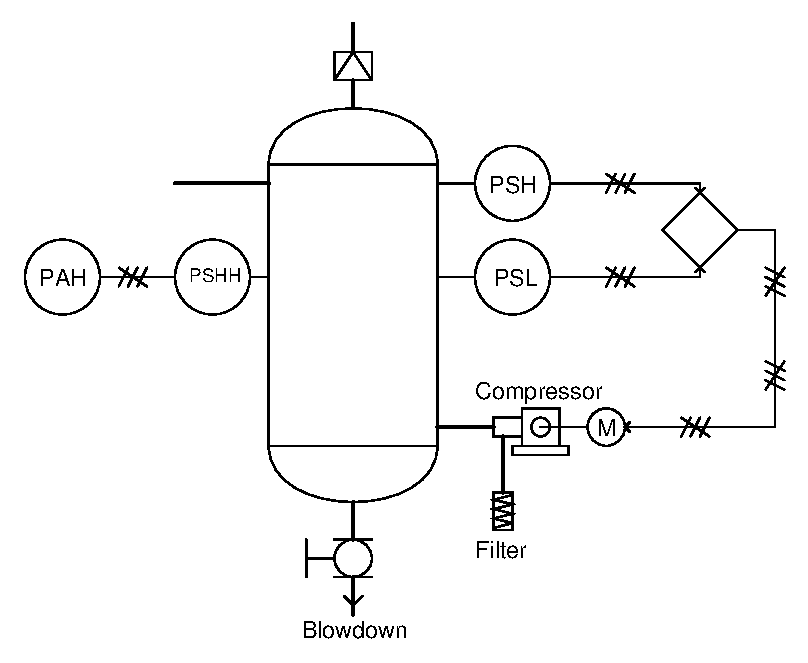
\includegraphics[width=15.5cm]{i00219x01.eps}$$

\underbar{file i00219}
%(END_QUESTION)





%(BEGIN_ANSWER)

Dette er et trykkreguleringssystem for en luftkompressor.  Det bruker to trykkbrytere, en høy (``PSH'') og en lav (``PSL''), som sender av/på-signaler til en logisk styrekrets (muligens en PLC).  Logikken slår deretter kompressormotoren av og på.

En sprengskive er montert på mottakertanken for avlastning ved høyt trykk, og en manuelt betjent kuleventil gir kontrollert utblåsning.

Boblen ``PSHH'' er en høy-høy-trykkbryter, som aktiveres bare når trykket i mottakertanken er over normalt driftstrykk.  Den sender et av/på-signal til en høytrykksalarmindikator (``PAH'').

%(END_ANSWER)





%(BEGIN_NOTES)

Pass på å spørre studentene spesifikt hvilke symboler som representerer alle elementene identifisert i svaret!

%INDEX% Process: air compressor and receiver tank
%INDEX% Switch, pressure: P&ID symbols

%(END_NOTES)
